\documentclass[a4paper,12pt]{article} % тип документа

\newcommand\nameone{Цыганкова Екатерина}
\newcommand\groupone{Б02-409}
\newcommand\labnumber{4.2.1}
\newcommand\labwork{Кольца Ньютона}
%%% Работа с русским языком
\usepackage{cmap}					% поиск в PDF
\usepackage{mathtext} 				% русские буквы в формулах
\usepackage[T2A]{fontenc}			% кодировка
\usepackage[utf8]{inputenc}			% кодировка исходного текста
\usepackage[main = russian, english]{babel}	% локализация и переносы
%\selectlanguage{english} (для англостатей)
%\usepackage{caption}

%%% Дополнительная работа с математикой
\usepackage{amsmath,amsfonts,amssymb,amsthm,mathtools} % AMS
\usepackage{icomma}
\usepackage{physics}
\usepackage{multicol}
\usepackage{bm}
\usepackage{mathrsfs}
\usepackage{verbatim}

%%% Номера формул
%\mathtoolsset{showonlyrefs=true} 
%\usepackage{leqno} 

%%% Свои команды
\DeclareMathOperator{\sgn}{sgn}

\usepackage{csquotes} 
\usepackage[backend=biber,style=authoryear]{biblatex}


%%% Работа с графикой
\usepackage{graphicx}
\graphicspath{{images/}}  
\setlength\fboxsep{3pt} 
\setlength\fboxrule{1pt} 
\usepackage{wrapfig} 
\usepackage{subcaption}
\usepackage{tikz}
\usepackage{pgfplots}
\usepackage{pgfplotstable}
\usepgfplotslibrary{polar}
\pgfplotsset{compat=1.18} 

%%% Работа с таблицами
\usepackage{array,tabularx,tabulary,booktabs}
\usepackage{longtable}  
\usepackage{multirow} 
\usepackage{soul} 

%%% Теоремы
\theoremstyle{plain} 
\newtheorem{theorem}{Th}[section]
\newtheorem{proposition}[theorem]{Proposition}
\newtheorem{question}{Question}[section]
 
\theoremstyle{definition} 
\newtheorem{corollary}{Corollary}[theorem]
\newtheorem{problem}{Problem}[section]
\newtheorem{definition}{Def}[section]
 
\theoremstyle{remark} 
\newtheorem*{nonum}{Solution}

%%% Программирование
\usepackage{etoolbox} 

%%% Гиперссылки
\usepackage{hyperref}

\usetikzlibrary{knots}
\usepackage{tcolorbox}

%%% Страница
\usepackage{geometry} 
	\geometry{top=20mm, bottom=20mm, left=15mm, right=20mm}

\usepackage{setspace} 

\usepackage{lastpage} 
\usepackage{amssymb}
\usepackage{xcolor}
\usepackage[all]{xy}
\usepackage{dsfont}



\begin{document}
\begin{center}   
	\large{Лабораторная работа № \labnumber\\ \hfill \break\Large{\textbf{\labwork}}}\\
    \normalsize
    \begin{flushright}
    \nameone, \groupone \\
    \today
    \end{flushright}
\end{center}
\begin{center}
Наблюдение интерференционной картины колец Ньютона позволяет измерять геометрические параметры линз или спектральный состав излучения. В работе по зависимости радиуса колец Ньютона в монохроматическом свете от их номера определяется радиус сферической поверхности плоско-выпуклой линзы. Анализ же видности картины в бихроматическом свете двух близких спектральных линий позволяет с хорошей точностью определить разность их длин волн.
\end{center}

\tableofcontents

\newpage
\section{Теоретические сведения}

В нашей установке кольца Ньютона образуются при интерференции световых волн, отражённых от границ тонкой воздушной прослойки, заключённой между выпуклой поверхностью линзы и плоской стеклянной пластинкой.
Линии постоянной разности хода представляют собой концентрические кольца с центром в точке соприкосновения. 
Если радиус соприкосновения линзы с пластинкой -- $r_0$, то радиусы тёмных и светлых колец определяются формулами \eqref{dark} и \eqref{light} соответственно.

\begin{equation}
    r_{dark}^2 - r_0^2 = m\lambda R
    \label{dark}
\end{equation}

\begin{equation}
    r_{light}^2-r_0^2 = (m - \frac{1}{2})\lambda R
    \label{light}
\end{equation}

\section{Экспериментальная установка}
Схема экспериментальной установки приведена на рис. \ref{ust}. Опыт выполнялся с помощью измерительного микроскопа. На столике микроскопа был помещен держатель с пластинкой из чёрного стекла. На пластинке -- исследуемая линза.

Источником света служила ртутная лампа Л, находящаяся в защитном кожухе. Для получения монохроматического света применялся монохроматор, состоящий из конденсора $K$ светофильтра $\Phi$ и объектива $O$, размещенных на оптической скамье. Свет от монохроматора попадал на опак-иллюминатор (ОИ), расположенный между окуляром и объективом микроскопа. Внутри опак-иллюминатора находилась полупрозрачная пластинка $P$, наклоненная под углом 45$^\circ$ к оптической оси микроскопа. Свет, частично отраженный от этой пластинки, проходил через объектив микроскопа и попадал на исследуемый объект.

Сначала микроскоп был настроен на кольца Ньютона в белом свете (Рис \ref{white}), а затем -- в выделенном монохроматором желтом или зеленом.

\begin{figure}[h]
    \centering
    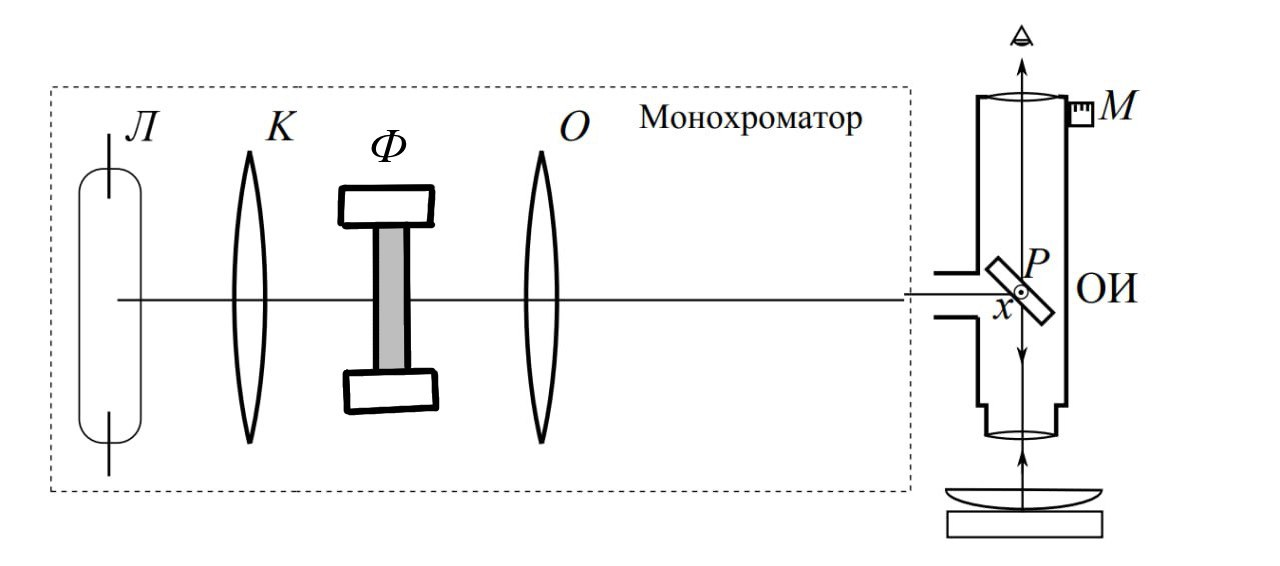
\includegraphics[width = 0.7\textwidth]{pics/установка.png}
    \caption{Схема установки для наблюдения колец Ньютона}
    \label{ust}
\end{figure}

\newpage
\begin{figure}[h]
\centering
\subcaptionbox{белый свет без фильтрации \label{white}}{
\includegraphics[width=0.3\textwidth]{pics/белый.jpg}}%
\hfill % <-- Seperation
\subcaptionbox{желтый ($\lambda_1 = 578$ нм) и зеленый ($\lambda_2 = 546$ нм) спектральные пики \label{green}}{
\includegraphics[width=0.3\textwidth]{pics/зеленый.jpg}}%
\hfill % <-- Seperation
\subcaptionbox{желтый дублет ($\lambda_1 = 578$ нм)\label{yellow}}{
\includegraphics[width=0.3\textwidth]{pics/желтый.jpg}}%
\caption{Сравнение четкости колец Ньютона при разной ширине спектра света.}
\label{photo}
\end{figure}

\section{Определение радиуса кривизны линзы}

\begin{wrapfigure}{r}{0.35\textwidth}
  \begin{center}
    
\includegraphics[width=0.34\textwidth]{pics/backlash.png}
  \end{center}
  \caption{Симметрия интерференционной картины}
  \label{backlash}
\end{wrapfigure}

Для определения радиуса кривизны линзы, был отфильтрован желтый спектральный пик ртутной лампы (Рис. \ref{yellow}). При помощи микрометрического винта, были измерены радиусы темных и светлых колец. Результаты измерений представлены в таблице \ref{rings}.

По этим данным был построен график зависимости квадрата радиуса темных и светлых колец (Рис. \ref{r_squared}) от номера кольца и, как следствие формул \eqref{dark} и \eqref{light}, вычислен радиус кривизны линзы. 
\[
\boxed{R = \frac{k}{\lambda} = 23,2 \pm 0,5 \text{ мм}} 
\]
где $\lambda = 578$ нм -- длина волны желтого пика в спектре ртути. 

Также по подъему графика согласно формулам \eqref{dark} и \eqref{light} был определен диаметр контакта линзы с пластинкой:

\[
\boxed{
    d = 2\sqrt{b_{dark}} = 2\sqrt{b_{light} + \frac{\lambda R}{2}} = (0,24 \pm 0,02) \text{ мм}
    }
\]

\begin{figure}[h]
    \centering
    
\includegraphics[width=0.9\linewidth]{pics/dark and light.png}
    \caption{Зависимость квадрата радиуса колец минимальной и максимальной иненсивности на интерференционной картине от их номера}
    \label{r_squared}
\end{figure}


\subsection{Оценка радиуса кривизны по фокусному расстоянию}
В качестве проверки полученного результата, освещая линзу далеким источником света, мы приблизительно нашли ее фокусное расстояние ($F \approx 5$ см). Для плоско-выпуклой стеклянной линзы $R = F(n - 1) \approx 25$ мм, что совпадает по порядку величины с измеренным значением.

\newpage
\subsection{Наблюдение биений}
При освещении системы светом, содержащим две спектральные компоненты, наблюдается характерная картина биений: чёткость интерференционных колец периодически изменяется (Рис. \ref{green}). Это объясняется наложением двух систем интерференционных колец, возникающих для разных длин волн $\lambda_1$ и $\lambda_2$. Число полос между центрами первой четкой системы до центра второй тогда определяется по формуле $\Delta m \approx \lambda_2/\Delta \lambda$, где $\Delta \lambda = \lambda_1 - \lambda_2$. 

В нашей работе для наблюдения биений использовались линии желтого ($\lambda_1 = 578$ нм) и зеленого ($\lambda_2 = 546$ нм) цветов. Полученное в эксперименте $\Delta m_{\text{эксп}} = 17 \pm 1$ совпало с теоретическим $\Delta m_{\text{теор}} = 17$.

\section{Заключение}

В работе было проведено наблюдение колец Ньютона в отраженном свете. По зависимости радиуса колец от их порядка был рассчитан радиус кривизны исследуемой линзы $R = 23,2 \pm 0,5 \text{ мм}$.

Также была получена интерференционная картина "биений", смешением зеленой и желтой линий спектра ртутной лампы. Характерное число полос за одно биение ($\Delta m_{\text{эксп}} = 17 \pm 1$) совпало с теоретическим ($\Delta m_{\text{теор}} = 17$).

\begin{table}[]
\centering
\begin{tabular}{|c|c|c|c|c|}
\hline
\textbf{\begin{tabular}[c]{@{}c@{}}$m$, номер\\ кольца\end{tabular}} & \textbf{\begin{tabular}[c]{@{}c@{}}$r_{dark}$, мкм\\ радиусы темных\\ колец\end{tabular}} & \textbf{$\sigma_{r_{dark}}$, мкм} & \textbf{\begin{tabular}[c]{@{}c@{}}$r_{light}$, мкм\\ радиусы светлых\\ колец\end{tabular}} & \textbf{$\sigma_{r_{light}}$, мкм} \\ \hline
1                                                                    & 165                                                                                       & 6                                 & 142                                                                                          & 11                                 \\ \hline
2                                                                    & 203                                                                                       & 5                                 & 185                                                                                          & 8                                  \\ \hline
3                                                                    & 234                                                                                       & 4                                 & 219                                                                                          & 7                                  \\ \hline
4                                                                    & 263                                                                                       & 4                                 & 248                                                                                          & 7                                  \\ \hline
5                                                                    & 288                                                                                       & 5                                 & 275                                                                                          & 5                                  \\ \hline
6                                                                    & 309                                                                                       & 3                                 & 300                                                                                          & 5                                  \\ \hline
7                                                                    & 328                                                                                       & 4                                 & 318                                                                                          & 5                                  \\ \hline
8                                                                    & 349                                                                                       & 4                                 & 338                                                                                          & 5                                  \\ \hline
9                                                                    & 369                                                                                       & 4                                 & 359                                                                                          & 4                                  \\ \hline
10                                                                   & 387                                                                                       & 4                                 & 378                                                                                          & 4                                  \\ \hline
11                                                                   & 402                                                                                       & 4                                 & 395                                                                                          & 4                                  \\ \hline
12                                                                   & 419                                                                                       & 4                                 & 410                                                                                          & 5                                  \\ \hline
13                                                                   & 433                                                                                       & 4                                 & 426                                                                                          & 4                                  \\ \hline
14                                                                   & 449                                                                                       & 4                                 & 441                                                                                          & 5                                  \\ \hline
15                                                                   & 466                                                                                       & 4                                 & 458                                                                                          & 5                                  \\ \hline
\end{tabular}
\caption{Зависимость радиуса темных и светлых колец от их номера}
\label{rings}
\end{table}
\end{document}